\documentclass[
	% -- opções da classe memoir --
	12pt,				% tamanho da fonte
	openright,			% capítulos começam em pág ímpar (insere página vazia caso preciso)
    twoside,			% para impressão em recto e verso. Oposto a oneside
	a4paper,			% tamanho do papel. 
	% -- opções da classe abntex2 --
	%chapter=TITLE,		% títulos de capítulos convertidos em letras maiúsculas
	%section=TITLE,		% títulos de seções convertidos em letras maiúsculas
	%subsection=TITLE,	% títulos de subseções convertidos em letras maiúsculas
	%subsubsection=TITLE,% títulos de subsubseções convertidos em letras maiúsculas
	% -- opções do pacote babel --
	english,			% idioma adicional para hifenização
	french,				% idioma adicional para hifenização
	spanish,			% idioma adicional para hifenização
	brazil				% o último idioma é o principal do documento
	]{abntex2}

\usepackage{lmodern}			% Usa a fonte Latin Modern			
\usepackage[T1]{fontenc}		% Selecao de codigos de fonte.
\usepackage[utf8]{inputenc}		% Codificacao do documento (conversão automática dos acentos)
\usepackage{lastpage}			% Usado pela Ficha catalográfica
\usepackage{indentfirst}		% Indenta o primeiro parágrafo de cada seção.
\usepackage{color}				% Controle das cores
\usepackage{graphicx}			% Inclusão de gráficos
\usepackage{microtype} 			% para melhorias de justificação

% math packages
\usepackage{amsmath}
\usepackage{amsfonts}
\usepackage{amssymb}
\usepackage{amsthm}

\usepackage{tikz, tkz-euclide}
\usetikzlibrary{babel}
\usetkzobj{all}

\theoremstyle{plain}
\newtheorem{example}{Exemplo}

\author{Eduardo José de Oliveira}
\title{Anotações:\\Método de Rayleigh-Ritz}

\setlength{\parindent}{1.3cm}
\setlength{\parskip}{0.2cm}

\newcommand{\todo}[1]{{\color{red}#1}}


\begin{document}

\maketitle

No cálculo variacional, procura-se uma função $y(x)$ que dentre as funções admissíveis torna o funcional estacionário. No método de Rayleigh-Ritz, a função $y(x)$ exata é substituida por uma função aproximada $v(x)$ formada por uma combinação linear de funções $\phi_i(x)$.

Note que, a escolha adequada das funções $\phi_i(x)$ é importante para se obter uma boa aproximação para a solução do problema.

Seja o funcional 
$$
	Y=\int_{x_1}^{x_2} f(x,y,y')dx\text{,}
$$ 
com as condições de contorno $y(x_1)=0$ e $y(x_2)=0$, então,
$$
	y(x) \approx 
	v(x) =
	\sum_{i=1}^{n} a_i \phi_i (x)
	\text{,}
$$
onde $\phi_i$ são chamadas funções de forma e devem ser linearmente independente, onde cada uma delas deve satisfazer as condições de contorno
$$
	\phi_i(x_1) = 
	\phi_i(x_2) = 
	0
	\text{,}
$$
para todo $i=1$, $2$, $3$, $\dots$

Essas funções são contínuas até o grau $m-1$, sendo $m$ a ordem da maior derivada do funcional. Os coeficientes $a_i$ são chamados parâmetros de deslocamento e, finalmente, $v(x)$ é chamada de função aproximadora.

Substituindo $y$ por $v$ no funcional $Y$ e aplicando a condição de estacionáriedade, $\delta Y=0$, tem-se
$$
	\delta Y = 
	\frac{\partial Y}{\partial a_i} \delta a_i
	+
	\frac{\partial Y}{\partial a_2} \delta a_2
	+ \cdots +
	\frac{\partial Y}{\partial a_n} \delta a_n
	= 0\text{.}
$$

Como as variações $\delta a_i$ são arbitrárias, a equação se transforma em um sistema de equações homogêneas da forma
$$
	\frac{\partial Y}{\partial a_i} = 0
	\text{,}
$$
onde $i=1$, $2$, $3$, $\dots$, $n$.

\begin{example}
	Considere a Viga prismática:
	\begin{figure}[h]
		\centering
		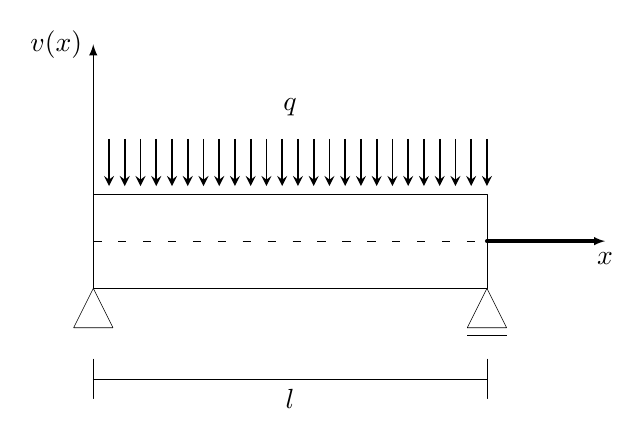
\begin{tikzpicture}
			\tkzInit[xmin=-0, xmax=6, ymin=-0.6, ymax=2]
			% draw axis without ticks
			\tkzDrawX[label=$x$, noticks, loosely dashed]
			\tkzDrawY[label=$v(x)$, noticks]
			
			% rectangle
			\tkzDefPoints{
				0/0.6/V_1,
				5/0.6/V_2,
				5/-0.6/V_3,
				0/-0.6/V_4}
			% complete x axis without dashed line
			\tkzDefPoints{
				5/0/A_1,
				6.35/0/A_2}
			% left base triangle
			\tkzDefPoints{
				0/-0.6/T1_1, 
				-0.25/-1.1/T1_2, 
				0.25/-1.1/T1_3}
			% right base triangle
			\tkzDefPoints{
				5/-0.6/T2_1, 
				4.75/-1.1/T2_2,
				5.25/-1.1/T2_3}
			% line on base of right triangle
			\tkzDefPoints{
				4.75/-1.2/T2_B1,
				5.25/-1.2/T2_B2}
			% length marker in bottom
			\tkzDefPoints{
				0/-1.5/L_1,
				0/-2/L_2,
				5/-1.5/L_3,
				5/-2/L_4,
				0/-1.75/LS_1,
				5/-1.75/LS_2}
			
			\tkzDrawSegment[color=black, line width=0.5mm](A_1, A_2)
			
			\tkzDrawPolygon[draw=black](T1_1, T1_2, T1_3)
			\tkzDrawPolygon[draw=black](T2_1, T2_2, T2_3)
			\tkzDrawSegment[color=black](T2_B1, T2_B2)
			\tkzDrawPolygon[draw=black](V_1, V_2, V_3, V_4)
			% q arrows
			\foreach \i in {1,...,25}{
				\tkzDefPoint(0.2*\i,1.3){A_\i}
				\tkzDefPoint(0.2*\i,0.7){B_\i}
				\draw[line width=0.6pt, black,-stealth] (A_\i) -- (B_\i);
			}
			% q text
			\node at (2.5,1.7) {$q$};
			% length marker in bottom
			\tkzDrawSegment[color=black](L_1, L_2)
			\tkzDrawSegment[color=black](L_3, L_4)
			\tkzDrawSegment[color=black](LS_1, LS_2)
			\node at (2.5,-2) {$l$};
		\end{tikzpicture}
	\end{figure}
	
	O funcional de energia potencial total associado ao problema da viga prismática é
	$$
		\Pi =
		\frac{1}{2}
		\int_0^l EI \left [ \frac{d^2 v}{dx^2} \right ]^2 dx
		-
		\int_0^l qvdx
		\text{,}
	$$
	onde $E$ é o módulo de Young do material e $I$ é o momento de inércia da seção transversal da viga em relação ao eixo baricêntrico.
	
	Como primeira aproximação, podemos utilizar a função $v_1(x)=a_0+a_1x+a_2x^2$, de onde, considerando as condições de contorno, tem-se que
	$$v_1(0)=0\Longrightarrow a_0=0\text{,}$$
	e de $v_1(l)=0$ concluí-se que $a_1=-a_2 l$. Assim, a função pode ser escrita como $$v_1(x)=a_2(x^2-lx) \text{.}$$
	
	Sua derivada é $v_1'(x)=a_2(2x-l)$ e, a derivada de segunda ordem é $v_1''(x)=2a_2$. Substituindo esses valores no funcional, tem-se que
	$$
		\Pi =
		\frac{1}{2}
		\int_0^l 4 EI a_2 ^2 dx
		-
		\int_0^l q a_2 (x^2-lx) dx
		\text{.}
	$$
	
	Da condição de estacionáriedade, $\delta \Pi=$, tem-se que
	$$
		\frac{\partial \Pi}{\partial a_0} \delta a_0
		+
		\frac{\partial \Pi}{\partial a_1} \delta a_1
		+
		\frac{\partial \Pi}{\partial a_2} \delta a_2
		= 0 \text{,}
	$$
	e, como $\Pi$ independe de $a_0$ e $a_1$, a equação se reduz a
	$$
		\frac{\partial \Pi}{\partial a_2} \delta a_2 
		= 0
		\text{,}
	$$
	de onde, devido ao fato de $\delta a_2$ ser arbitrário, obtem-se a equação
	$$
		\frac{\partial \Pi}{\partial a_2} = 0
	$$
	$$
		\frac{\partial \Pi}{\partial a_2}
		=
		\frac{\partial}{\partial a_2} \left [
			\int_0^l \left ( 2EIa_2 ^2 - a_2 q (x^2 -lx) \right ) dx
		\right]
	$$
	$$
		\frac{\partial \Pi}{\partial a_2}
		=
		\int_0^l
			\frac{\partial}{\partial a_2} \left [
			4EIa_2^2 - a_2 q(x^2-lx)
		\right ] dx
	$$
	$$
		\frac{\partial \Pi}{\partial a_2}
		=
		\int_0^l \left [
			4EIa_2 - q(x^2-lx)
		\right ] dx = 0
	$$
	$$
		\left [ 
			4EIa_2 x \Big |_0^l
			-
			q \left (
				\frac{x^3}{3} - \frac{lx^2}{2}
			\right ) \Big |_0^l
		\right ] 
		= 0
	$$
	$$
		4EIa_2l
		-
		q \left (\frac{l^3}{3} - \frac{l^3}{2} \right )
		= 0
	$$	
	$$
		4EIa_2l+\frac{ql^3}{6} = 0
	$$
	$$
		a_2=\frac{-ql^2}{24EI}\text{.}
	$$

	Com o valor de $a_2$ é possível calcular o valor de $a_1=-a_2l$, então, 
	$$a_1=\frac{ql^3}{24EI}\text{.}$$
	
	Assim, a função aproximadora $v_1$ pode ser escrita como
	$$
		v_1(x)=
		\frac{ql^3}{24EI}x
		-
		\frac{ql^2}{24EI}x^2
		\text{.}
	$$
	
	Pode-se utilizar uma aproximação de grau 3 para tentar melhorar o resultado, isto é, $v_2(x)=a_0+a_1x+a_2x^2+a_3x^3$. Das condições de contorno, $v_2(0)=0$, de onde $a_0=0$ e $v_2(l)=0$, donde $a_1=-a_2 l - a_3 l^2$. Assim, a função pode ser escrita como
	$$
		v_2(x)=
		a_2(x^2-lx)
		+
		a_3(x^3-l^2x)
		\text{.}
	$$
	
	Das condições de contorno, tem-se que $v_2(0)=0$, donde pode-se concluir que $a_0=0$. Ainda, $v_2(l)=0$, de onde, $a_1 l + a_2 l^2 + a_3 l^3=0$, isto é, $a_1=-a_2 l - a_3 l^2$. Assim, a função pode ser reescrita como
	$$
		v_2(x)=
		a_2(x^2-lx)
		+
		a_3(x^3-l^2x)
		\text{.}
	$$
	
	Derivando a função $v_2$ em função de x, pode-se obter
	$$
	v_2'(x)=
	a_2(2x-l)
	+
	a_3(3x^2-l^2)
	$$

	$$
	v_2''(x)=
	2a_2 + 6a_3 x \text{.}
	$$
	
	Substituindo em $\Pi$, tem-se
	$$
		\Pi=
		\frac{1}{2}
		\int_0^l
			\left (
				EI(2a_2+6a_3x)^2
			\right ) dx
		-
		\int_0^l
			q
			\left (
				a_2(x^2-lx)
				+
				a_3(x^3-l^2x)
			\right ) dx
		\text{.}
	$$
	
	Derivando $\Pi$ em função de $a_2$ é possível obter
	$$
		\frac{\partial \Pi}{\partial a_2}
		=
		\int_0^l \left [
			2EI(2a_2+6a_3x)-q(x^2-lx)
		\right ] dx
		= 0
	$$	
	$$
		\frac{\partial \Pi}{\partial a_2}
		=
		\int_0^l \left [
			EI(4a_2+12a_3x)-q(x^2-lx)
		\right ] dx
		= 0
	$$
	$$
		\int_0^l \left [
			4EIa_2 + 12EIa_3x - qx^2 + qlx
		\right ] dx
		= 0
	$$
	$$
		4EIa_2 x \Big |_0^l
		+
		\frac{12a_3EI}{2} x^2 \Big |_0^l
		-
		\frac{q}{3} x^3 \Big |_0^l
		+
		\frac{ql}{2} x^2 \Big |_0^l
		= 0
	$$
	$$
		4EIa_2l
		+
		6a_3EIl^2
		-
		\frac{2ql^3}{6}
		+
		\frac{3ql^3}{6}
		= 0
	$$
	$$
		4EIa_2l
		+
		6a_3EIl^2
		=
		\frac{2ql^3}{6}
		-
		\frac{3ql^3}{6}
	$$
	$$
		4a_2 + 6a_3l
		=
		\frac{-ql^2}{6EI}
	$$
	\begin{equation}
		\label{eq:approx2_eq1}
		2a_2 + 3a_3l
		=
		\frac{-ql^2}{12EI}
		\text{.}
	\end{equation}
	
	Derivando $\Pi$ em relação a $a_3$ tem-se que
	$$
		\frac{\partial \Pi}{\partial a_3}
		=
		\int_0^l \left [
			6EI(2a_2 + 6a_3x)x
			-
			q(x^3 - l^2x)
		\right ] dx
		= 0
	$$
	$$
		\int_0^l \left [
			EI(12a_2 + 36a_3x)x
			-
			q(x^3 - l^2x)
		\right ] dx
		= 0
	$$
	$$
		\int_0^l \left [
			EI(12a_2 x + 36a_3x^2)
			-
			q(x^3 - l^2x)
		\right ] dx = 0
		= 0
	$$
	$$
		EI \left (
			\frac{12a_2}{2}x^2 \Big |_0^l
			+
			\frac{36a_3}{3}x^3 \Big |_0^l
		\right )
		-
		q \left (
			\frac{x^4}{4} \Big |_0^l
			-
			\frac{l^2x^2}{2} \Big |_0^l
		\right )
		= 0
	$$
	$$
		EI(6a_2l^2 + 12a_3l^3)
		-
		q \left (
			\frac{l^4}{4}
		\right )
		+
		q \left (
			\frac{l^4}{2}
		\right )
	$$
	$$
		6a_2 + 12a_3l = -\frac{ql^4}{4EIl^2}
	$$
	$$
		6a_2 + 12a_3l = -\frac{ql^2}{4EI}
	$$
	\begin{equation}
		\label{eq:approx2_eq2}
		2a_2 + 4a_3l = -\frac{ql^2}{12EI}
		\text{.}
	\end{equation}
	
	Montando um sistema de equações com \eqref{eq:approx2_eq1} e \eqref{eq:approx2_eq2} é possível encontrar os valores de $a_2$ e $a_3$. Fazendo \eqref{eq:approx2_eq2} - \eqref{eq:approx2_eq1}, tem-se $2a_2+4a_3l-2a_2-3a_3l=-\frac{ql^2}{12EI}+\frac{ql^2}{12EI}$, donde $a_3l=0$ e, então, $a_3=0$.
	De volta a \eqref{eq:approx2_eq1}, substituindo $a_3=0$, reduzimos a equação a $2a_2=-\frac{ql^2}{12EI}$ e, por fim,
	$$
		a_2=-\frac{ql^2}{24EI}
		\text{.}
	$$
	Assim, a função $v_2$ é a mesma que $v_1$, não sendo muito útil ao caso.
	
	Utilizando, como função aproximadora, a função $v_3(x)=a_0+a_1x+a_2x^2+a_3x^3+a_4x^4$, tem-se das condições de contorno que $v_3(0)=0$, donde $a_0=0$ e, $v_3(l)=0$, isto é $a_1l+a_2l^2+a_3l^3+a_4l^4=0$, donde pode-se concluir que $a_1=-a_2l-a_3l^2-a_4l^3$. Substituindo $a_0$ e $a_1$ em $v_3(x)$, podemos encontrar a função
	$$
		a_2 (x^2 - lx)
		+
		a_3 (x^3 - l^2x)
		+
		a_4 (x^4 - l^3x)
		\text{.}
	$$
	
	Derivando $v_3$ em relação a $x$:
	$$
		v_3'(x)=
		a_2(2x - l)
		+
		a_3(3x^2 - l^2)
		+
		a_4(4x^3 - l^3)
	$$
	$$
		v_3''(x)=
		2a_2
		+
		6a_3 x
		+
		12a_4 x^2
		\text{.}
	$$
	
	Substituindo em $\Pi$,
	$$
		\Pi = \frac{1}{2} \int_0^l \left [
			EI(2a_2+6a_3x+12a_4x^2)^2
		\right ] dx
		-
		\int_0^l q \left [
			a_2(x^2 - lx)
			+
			a_3(x^3 - l^2x)
			+
			a_4(x^4 - l^3x)
		\right ] dx
		\text{,}
	$$
	de onde pode-se derivar $\Pi$ em relação a $a_2$, $a_3$ e $a_4$ para obter um sistema de equações permitindo a determinação de $a_2$, $a_3$ e $a_4$.
	
	Fazendo $\frac{\partial \Pi}{\partial a_2} = 0$:
	$$
		\frac{\partial \Pi}{\partial a_2}
		=
		\int_0^l \left [
			2EI(2a_2 + 6a_3x + 12a_4x^2)
			-
			q(x^2 - lx)
		\right ] dx
		= 0
	$$
	$$
		\int_0^l \left [
			EI(4a_2 + 12a_3x + 24a_4x^2)
			-
			q(x^2 - lx)
		\right ] dx
		= 0
	$$
	$$
		EI \left (
			4a_2 x \Big |_0^l
			+
			\frac{12a^3}{2}x^2 \Big |_0^l
			+
			\frac{24a_4}{3}x^3 \Big |_0^l
		\right )
		- q
		\left (
			\frac{x^3}{3} \Big |_0^l
			-
			\frac{lx^2}{2} \Big |_0^l
		\right )
		= 0
	$$
	$$
		EI(4a_2l + 6a_3l^2 + 8a_4l^3)
		=
		\frac{ql^3}{3}
		-
		\frac{ql^3}{2}
	$$
	$$
		4a_2l + 6a_3l^2 + 8a_4l^3 = -\frac{ql^3}{6EI}
	$$
	\begin{equation}
		2a_2 + 3a_3l + 4a_4l^2 = -\frac{ql^2}{12EI}
		\text{.}
	\end{equation}
		
	Fazendo $\frac{\partial \Pi}{\partial a_3} = 0$:
		
\end{example}

\end{document}